% =================================================================================
% JEEVA KRISHNASAMY — CV (ENGLISH VERSION)
% Target: Formel AI — AI Engineer (LLMs + Formal Verification)
% Compile: xelatex (twice). Requires: lato, fontawesome5, accsupp.
% Place photo1.jpeg next to this file.
% =================================================================================

\documentclass[10pt,a4paper]{article}

\usepackage[left=1cm,top=1cm,right=1cm,bottom=0.55cm,nohead,nofoot]{geometry}
\usepackage[utf8]{inputenc}
\usepackage[T1]{fontenc}
\usepackage[english]{babel}
\usepackage[default]{lato}
\usepackage{fontawesome5}
\usepackage{tikz}
\usepackage{xcolor}
\usepackage{amssymb}
\usepackage{parskip}
\usepackage{enumitem}
\usepackage{accsupp}
\usepackage{hyperref}

\definecolor{primaryblue}{HTML}{1E3A8A}
\definecolor{accentblue}{HTML}{3B82F6}
\definecolor{sidebargrey}{HTML}{F8FAFC}
\definecolor{textgrey}{HTML}{1E293B}
\definecolor{lighttext}{HTML}{64748B}

\hypersetup{
    colorlinks=true, linkcolor=primaryblue, urlcolor=primaryblue, pdfborder={0 0 0},
    pdftitle={Resume - Jeeva Krishnasamy - Data \& AI Engineer},
    pdfauthor={Jeeva Krishnasamy},
    pdfkeywords={AI Engineer, LLM, RAG, Data Engineer, Python, PyTorch, Airflow, AWS}
}

% --- Icons hidden from ATS text extraction ---
\newcommand{\icon}[1]{\BeginAccSupp{ActualText={}}#1\EndAccSupp{}}

% --- Placeholders (red) ---
\newif\ifshowplaceholders
\showplaceholderstrue
\newcommand{\ph}[1]{\ifshowplaceholders\textcolor{red}{\textbf{[#1]}}\else\PackageError{CV}{Unfilled field: #1}{}\fi}

% --- Section titles ---
\newcommand{\sidesection}[2]{%
    \subsection*{\color{primaryblue}\icon{#1}\ #2}
    \vspace{-0.4cm}
    \textcolor{accentblue}{\rule{4.5cm}{0.5pt}}
}
\newcommand{\mainsection}[2]{%
    \section*{\color{primaryblue}\icon{#1}\ #2}
    \vspace{-0.6cm}
    \textcolor{accentblue}{\rule{14cm}{0.8pt}}
}
% --- Job header ---
\newcommand{\job}[3]{%
    {\fontsize{11}{13}\selectfont\textbf{#1}}\\
    \textsl{\color{lighttext}#2} \hfill \textit{\color{lighttext}#3}
}


\setlist[itemize]{itemsep=0.05em, topsep=0.1em}

\begin{document}
\pagestyle{empty}

% ============= BACKGROUND, PHOTO, NAME BANNER =============
\begin{tikzpicture}[remember picture,overlay]
    \fill[sidebargrey] (current page.north west) rectangle ([xshift=6cm]current page.south west);
    \fill[primaryblue] ([xshift=6cm, yshift=-4.3cm]current page.north west) rectangle (current page.north east);

    \node[anchor=north west, inner sep=0pt, xshift=1cm, yshift=-0.4cm] at (current page.north west) {
        \begin{tikzpicture}
            \clip (2.5cm, 2.5cm) circle (2.cm);
            \node[anchor=center] at (2.5cm, 2.2cm) {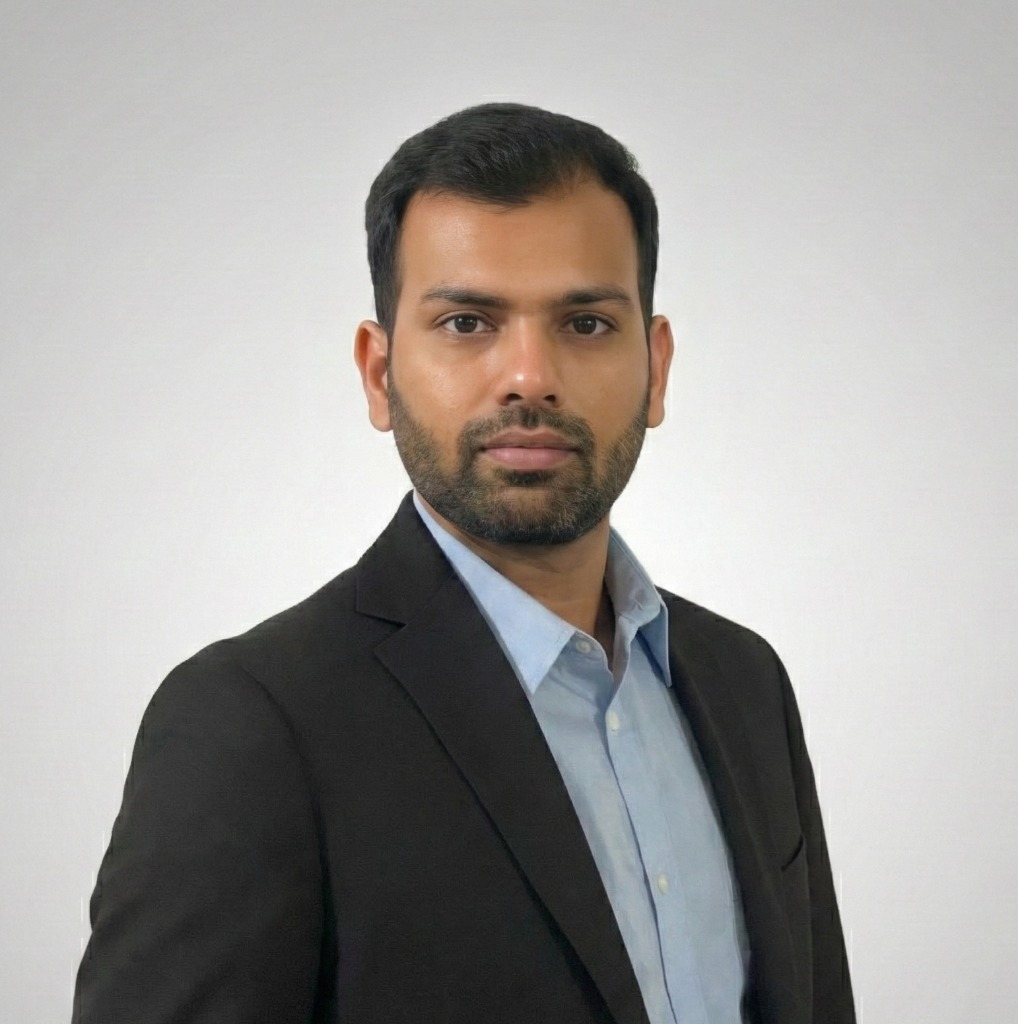
\includegraphics[width=5cm, height=5cm, keepaspectratio]{photo1.jpeg}};
        \end{tikzpicture}
    };

    \node[anchor=west, xshift=6.6cm, yshift=-2.2cm] at (current page.north west) {
        \begin{minipage}{13cm}
            \color{white}
            {\fontsize{34}{40}\selectfont \textbf{Jeeva Krishnasamy}}\\[0.4em]
            {\fontsize{14}{17}\selectfont Data \& AI Engineer --- LLM, RAG, Computer Vision}\\[0.3em]
            {\fontsize{10}{12}\selectfont French Talent Passport (no sponsorship required) \textbullet{} Available immediately}
        \end{minipage}
    };
\end{tikzpicture}

\vspace*{4.5cm}

\noindent
% ============= LEFT SIDEBAR =============
\begin{minipage}[t]{6.6cm}
    \raggedright
    \vspace{-1.17cm}

    \begin{minipage}[t]{4.6cm}
        \sidesection{\faAddressCard}{Contact}
        \vspace{-0.3cm}

        \small \color{textgrey}
        {\color{lighttext}\icon{\faPhone}} \ \ +33 7 44 29 08 23 \\[0.35em]
        {\color{lighttext}\icon{\faEnvelope}} \ \ \href{mailto:jivanandham@gmail.com}{jivanandham@gmail.com} \\[0.35em]
        {\color{lighttext}\icon{\faMapMarker*}} \ \ Poitiers, France \\[0.35em]
        {\color{lighttext}\icon{\faLinkedin}} \ \ \href{https://linkedin.com/in/jivanandham}{linkedin.com/in/jivanandham} \\[0.35em]
        {\color{lighttext}\icon{\faGithub}} \ \ \href{https://github.com/jivanandham}{github.com/jivanandham} \\[0.35em]
        {\color{lighttext}\icon{\faIdCard}} \ \ Talent Passport (no sponsorship) \\[0.35em]
    \end{minipage}

    \vspace{0.3cm}

    \begin{minipage}[t]{4.6cm}
        \sidesection{\faCogs}{Skills}
        \vspace{-0.3cm}

        \small \color{textgrey}\raggedright
        \textbf{\color{primaryblue}LLM \& Generative AI}
        \begin{itemize}[leftmargin=0.4cm, label={\color{accentblue}\tiny$\blacktriangleright$}]
            \item RAG, semantic re-ranking
            \item LangChain, ChromaDB
            \item LLM APIs
            \item Model evaluation
        \end{itemize}
        \vspace{0.1cm}

        \textbf{\color{primaryblue}ML \& Deep Learning}
        \begin{itemize}[leftmargin=0.4cm, label={\color{accentblue}\tiny$\blacktriangleright$}]
            \item PyTorch, TensorFlow
            \item Scikit-learn, NumPy, SciPy
            \item YOLOv8, RF-DETR
            \item Computer vision
            \item Predictive maintenance
        \end{itemize}
        \vspace{0.1cm}

        \textbf{\color{primaryblue}Data Engineering}
        \begin{itemize}[leftmargin=0.4cm, label={\color{accentblue}\tiny$\blacktriangleright$}]
            \item Python, SQL, Pandas
            \item Apache Airflow, ETL
            \item FastAPI, REST APIs, React.js
        \end{itemize}
        \vspace{0.1cm}

        \textbf{\color{primaryblue}Industrial Automation}
        \begin{itemize}[leftmargin=0.4cm, label={\color{accentblue}\tiny$\blacktriangleright$}]
            \item SCADA, PLC, IoT
        \end{itemize}
        \vspace{0.1cm}

        \textbf{\color{primaryblue}Cloud \& MLOps}
        \begin{itemize}[leftmargin=0.4cm, label={\color{accentblue}\tiny$\blacktriangleright$}]
            \item AWS, Docker, GPU/CUDA
            \item Linux, Bash, Git, CI/CD
        \end{itemize}
    \end{minipage}

    \vspace{0.5cm}

    \begin{minipage}[t]{4.6cm}
        \sidesection{\faLanguage}{Languages}
        \vspace{-0.3cm}

        \small \color{textgrey}
        \textbf{English}: fluent\\[0.3em]
        \textbf{French}: A2, improving\\[0.3em]
        \textbf{Tamil}: native
    \end{minipage}

    \vspace{0.5cm}

    \begin{minipage}[t]{4.6cm}
        \sidesection{\faCertificate}{Certification}
        \vspace{-0.3cm}

        \small \color{textgrey}
        \textbf{AWS Certified Solutions Architect}\\
        {\color{lighttext}\small Amazon Web Services, 2024}
    \end{minipage}

\end{minipage}%
\hspace{-1.1cm}%
% ============= MAIN COLUMN =============
\begin{minipage}[t]{14.0cm}
    \color{textgrey}
    \vspace{-1.8cm}

    \mainsection{\faUser}{Professional Summary}
    \vspace{-0.3cm}

    Data \& AI Engineer with 10+ years of engineering and data experience, including 2 years building production AI applications (LLM/RAG assistant, YOLOv8/RF-DETR object detection). Strong data engineering foundation (Airflow, ETL, SQL, AWS) to take models into reliable production.

    \vspace{-0.45cm}

    \mainsection{\faBriefcase}{Professional Experience}
    \vspace{-0.3cm}

    \job{AI Projects \& Training}{Poitiers, France}{Feb 2026 -- Present}
    \begin{itemize}[leftmargin=0.6cm, label={\color{accentblue}$\bullet$}]
        \item Building personal AI projects; taking French language classes (A2, improving).
    \end{itemize}
    \vspace{0.02cm}

    \job{Data Engineer \textmd{(alongside Master's)}}{University of Pittsburgh, USA}{Sep 2024 -- Jan 2026}
    \begin{itemize}[leftmargin=0.6cm, label={\color{accentblue}$\bullet$}]
        \item Built a RAG Slack assistant (LangChain, vector search, semantic re-ranking) deployed across \textbf{15 channels}, used by \textbf{1,500 students} (100 per channel) and 15 staff members.
        \item Built Python ETL pipelines (Coursera, Salesforce APIs) and 10+ production Airflow workflows with failure recovery, cutting manual maintenance by \textbf{40 hrs/week}.
    \end{itemize}
    \vspace{0.02cm}

    \job{AI Software Engineer \textmd{(Intern)}}{Airoverse, USA}{Mar 2024 -- May 2024}
    \begin{itemize}[leftmargin=0.6cm, label={\color{accentblue}$\bullet$}]
        \item Trained and deployed object detection models (YOLOv8, RF-DETR) in PyTorch, achieving \textbf{90\% precision} and \textbf{80\% recall} on production images.
        \item Built an end-to-end detection platform (FastAPI, React.js) and a real-time inference pipeline integrating Google Maps and Roboflow APIs, reducing manual processing by \textbf{90\%}.
    \end{itemize}
    \vspace{0.02cm}

    \job{Data \& Automation Engineer}{Shraddha Engineering, India}{Jun 2020 -- Dec 2022}
    \begin{itemize}[leftmargin=0.6cm, label={\color{accentblue}$\bullet$}]
        \item Led end-to-end deployment of automation systems and dashboards, saving \textbf{2,000+ engineering hours} per year.
        \item Built Python/SQL ETL pipelines harmonizing heterogeneous data; developed real-time monitoring software with alerts and REST APIs.
    \end{itemize}
    \vspace{0.02cm}

    \job{Systems \& Analytics Engineer}{Bluestar Limited, India}{Apr 2018 -- Jun 2020}
    \begin{itemize}[leftmargin=0.6cm, label={\color{accentblue}$\bullet$}]
        \item Developed predictive maintenance and statistical models in Python for industrial equipment, reducing failures by \textbf{22\%}.
        \item Coordinated a cross-functional team of \textbf{10} engineers deploying analytics solutions across multiple sites.
    \end{itemize}
    \vspace{0.02cm}

    \job{Automation Engineer}{Chennai Engineering Services, India}{Jun 2015 -- Apr 2018}
    \begin{itemize}[leftmargin=0.6cm, label={\color{accentblue}$\bullet$}]
        \item Automated data acquisition and reporting for industrial clients (Python, SQL), improving reliability by \textbf{15\%}.
        \item Developed PLC control logic integrated with business systems; cut project delivery times by \textbf{10\%}.
    \end{itemize}
    \vspace{0.02cm}

    \job{Apprentice Engineer \textmd{(Digital Monitoring)}}{TANGEDCO, India}{Mar 2014 -- Mar 2015}
    \begin{itemize}[leftmargin=0.6cm, label={\color{accentblue}$\bullet$}]
        \item Supported SCADA/IoT rollout on 5+ substations (200+ monitored assets) and digital metering, raising field efficiency by \textbf{35\%}.
    \end{itemize}

    \vspace{-0.45cm}

    \mainsection{\faGraduationCap}{Education}
    \vspace{-0.3cm}

    \job{Master of Science --- Information Science}{University of Pittsburgh, USA}{2023 -- 2025}\par
    {\small Project: deepfake detection with a ResNet CNN (cyber forensics) --- \href{https://github.com/jivanandham/Cyber-Forensics-Deepfake-Detection}{\icon{\faGithub}\ GitHub}}
    % Add an LLM project here (agent, fine-tuning, evaluation) once it is on GitHub.

    \vspace{0.1cm}

    \job{Bachelor of Engineering (B.E.) --- Electrical Engineering}{Anna University, India}{2009 -- 2013}

\end{minipage}

\end{document}